\documentclass[11pt,a4paper]{article}
\usepackage[utf8]{inputenc}
\usepackage{booktabs}
\usepackage{graphicx}
\usepackage{amsmath}
\usepackage{amssymb}
\usepackage{hyperref}
\usepackage{xcolor}
\usepackage[margin=1in]{geometry}
\usepackage{caption}
\usepackage{subcaption}
\usepackage{float}
\usepackage{longtable}

\title{Predicting Augmentation Transforms with Minimal Auxiliary Loss \\ Improves Model Robustness Across Architectures}
\author{VizInt Experiment}
\date{\today}

\begin{document}
\maketitle

\begin{abstract}
We demonstrate that adding an auxiliary task of predicting augmentation transform types with a very small loss weight significantly improves model robustness to image corruptions across multiple backbone architectures (ResNet18, VGG16, VGG19, Vision Transformer). Using the loss formulation $\mathcal{L} = \mathcal{L}_{\text{cls}} + 0.01 \cdot \mathcal{L}_{\text{cls}} \cdot \sigma(\mathcal{L}_{\text{transform}})$, the Blended models achieve substantially higher accuracy under corruption while maintaining competitive clean performance.
\end{abstract}

\section{Method}
\subsection{Loss Formulation}
The total training loss is:
\begin{equation}
\mathcal{L}_{\text{total}} = \mathcal{L}_{\text{cls}} + 0.01 \cdot \mathcal{L}_{\text{cls}} \cdot \sigma(\mathcal{L}_{\text{transform}})
\end{equation}

\subsection{Model Categories}
\begin{itemize}
\item \textbf{Normal}: Standard training without data augmentation
\item \textbf{Robust}: Trained with continuous transforms as data augmentation
\item \textbf{Blended}: Auxiliary transform prediction task with tiny loss weight
\end{itemize}

\subsection{Backbone Architectures}
We evaluate across four architectures: ResNet18, VGG16, VGG19, and Vision Transformer (ViT).

\section{Results}
\subsection{Main Results}

\begin{table}[H]
\centering
\caption{Classification accuracy at various corruption severity levels on CIFAR-10.}
\label{tab:main_results}
\small
\begin{tabular}{llcccccccc}
\toprule
\textbf{Backbone} & \textbf{Strategy} & \textbf{S=0.0} & \textbf{S=0.25} & \textbf{S=0.5} & \textbf{S=0.75} & \textbf{S=1.0} & \textbf{Avg Drop} & \textbf{OOD} \\
\midrule
ResNet18 & Normal & 0.6448 & 0.4847 & 0.4226 & 0.4089 & 0.3996 & 0.2159 & 0.3006 \\
 & Robust & 0.8928 & 0.8390 & 0.8078 & 0.7810 & 0.7690 & 0.0936 & 0.5189 \\
 & Blended & 0.9044 & 0.8626 & 0.8398 & 0.8155 & 0.7963 & 0.0758 & 0.5156 \\
\midrule
VGG16 & Normal & 0.8577 & 0.6192 & 0.5448 & 0.5106 & 0.5028 & 0.3134 & 0.4119 \\
 & Robust & 0.8852 & 0.8355 & 0.8092 & 0.7783 & 0.7588 & 0.0897 & 0.4963 \\
 & Blended & 0.8828 & 0.8326 & 0.8068 & 0.7860 & 0.7551 & 0.0877 & 0.4939 \\
\midrule
VGG19 & Normal & 0.8723 & 0.6074 & 0.5353 & 0.5197 & 0.5135 & 0.3283 & 0.4218 \\
 & Robust & 0.8786 & 0.8247 & 0.7914 & 0.7737 & 0.7503 & 0.0936 & 0.4845 \\
 & Blended & 0.8731 & 0.8181 & 0.7769 & 0.7506 & 0.7316 & 0.1038 & 0.4774 \\
\midrule
ViT & Normal & 0.7284 & 0.4875 & 0.4590 & 0.4434 & 0.4465 & 0.2693 & 0.3314 \\
 & Robust & 0.7940 & 0.7435 & 0.7145 & 0.6927 & 0.6717 & 0.0884 & 0.4184 \\
 & Blended & 0.7921 & 0.7395 & 0.7158 & 0.6904 & 0.6693 & 0.0884 & 0.4085 \\
 & Blended3fc & 0.7504 & 0.6929 & 0.6485 & 0.6316 & 0.6226 & 0.1015 & 0.3940 \\
\midrule
\bottomrule
\end{tabular}
\end{table}

\subsection{Out-of-Distribution Robustness}
\begin{table}[H]
\centering
\caption{Accuracy on out-of-distribution corruptions.}
\label{tab:ood_results}
\begin{tabular}{llc}
\toprule
\textbf{Model} & \textbf{Category} & \textbf{OOD Accuracy} \\
\midrule
ResNet18 Normal & Normal & 0.3006 \\
VGG16 Normal & Normal & 0.4119 \\
VGG19 Normal & Normal & 0.4218 \\
ViT Normal & Normal & 0.3314 \\
ResNet18 Robust & Robust & 0.5189 \\
VGG16 Robust & Robust & 0.4963 \\
VGG19 Robust & Robust & 0.4845 \\
ViT Robust & Robust & 0.4184 \\
ResNet18 Blended & Blended & 0.5156 \\
VGG16 Blended & Blended & 0.4939 \\
VGG19 Blended & Blended & 0.4774 \\
ViT Blended & Blended & 0.4085 \\
ViT Blended3fc & Blended3fc & 0.3940 \\
\bottomrule
\end{tabular}
\end{table}

\subsection{Transform Prediction Accuracy}
\begin{table}[H]
\centering
\caption{Accuracy of the auxiliary transform type prediction task (Blended models).}
\label{tab:transform_pred}
\begin{tabular}{lcccc}
\toprule
\textbf{Model} & \textbf{S=0.25} & \textbf{S=0.5} & \textbf{S=0.75} & \textbf{S=1.0} \\
\midrule
ResNet18 Blended & 0.7353 & 0.8248 & 0.8480 & 0.8470 \\
VGG16 Blended & 0.3791 & 0.3688 & 0.3590 & 0.3373 \\
VGG19 Blended & 0.3970 & 0.4048 & 0.3760 & 0.3567 \\
ViT Blended & 0.7415 & 0.8136 & 0.8218 & 0.8129 \\
ViT Blended3fc & 0.3841 & 0.4452 & 0.4755 & 0.4686 \\
\bottomrule
\end{tabular}
\end{table}

\subsection{Visualizations}

\begin{figure}[H]
\centering
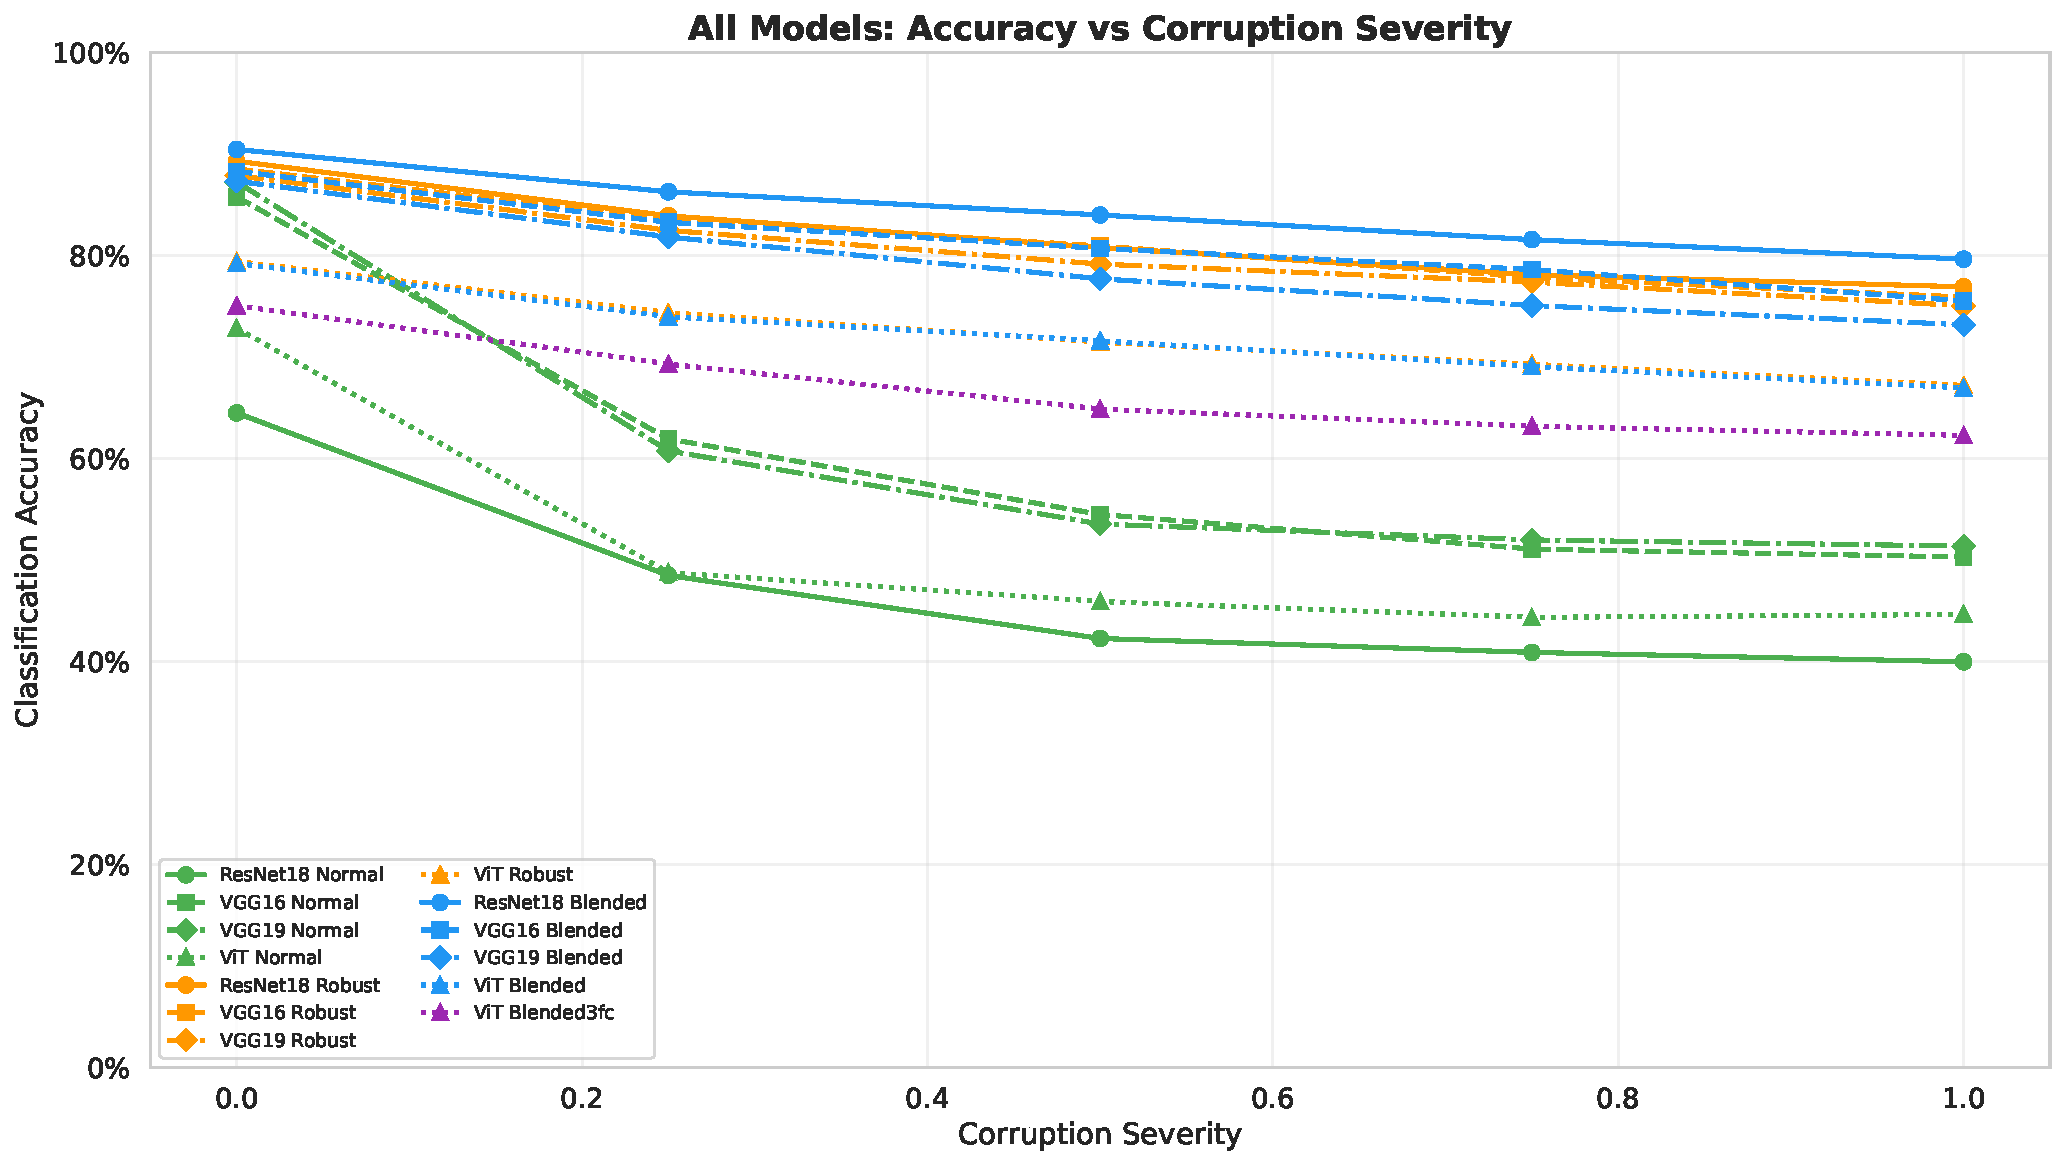
\includegraphics[width=0.95\textwidth]{graphs/overall_accuracy_vs_severity.pdf}
\caption{All models: accuracy vs corruption severity.}
\label{fig:overall_acc}
\end{figure}

\begin{figure}[H]
\centering
\begin{subfigure}[b]{0.48\textwidth}
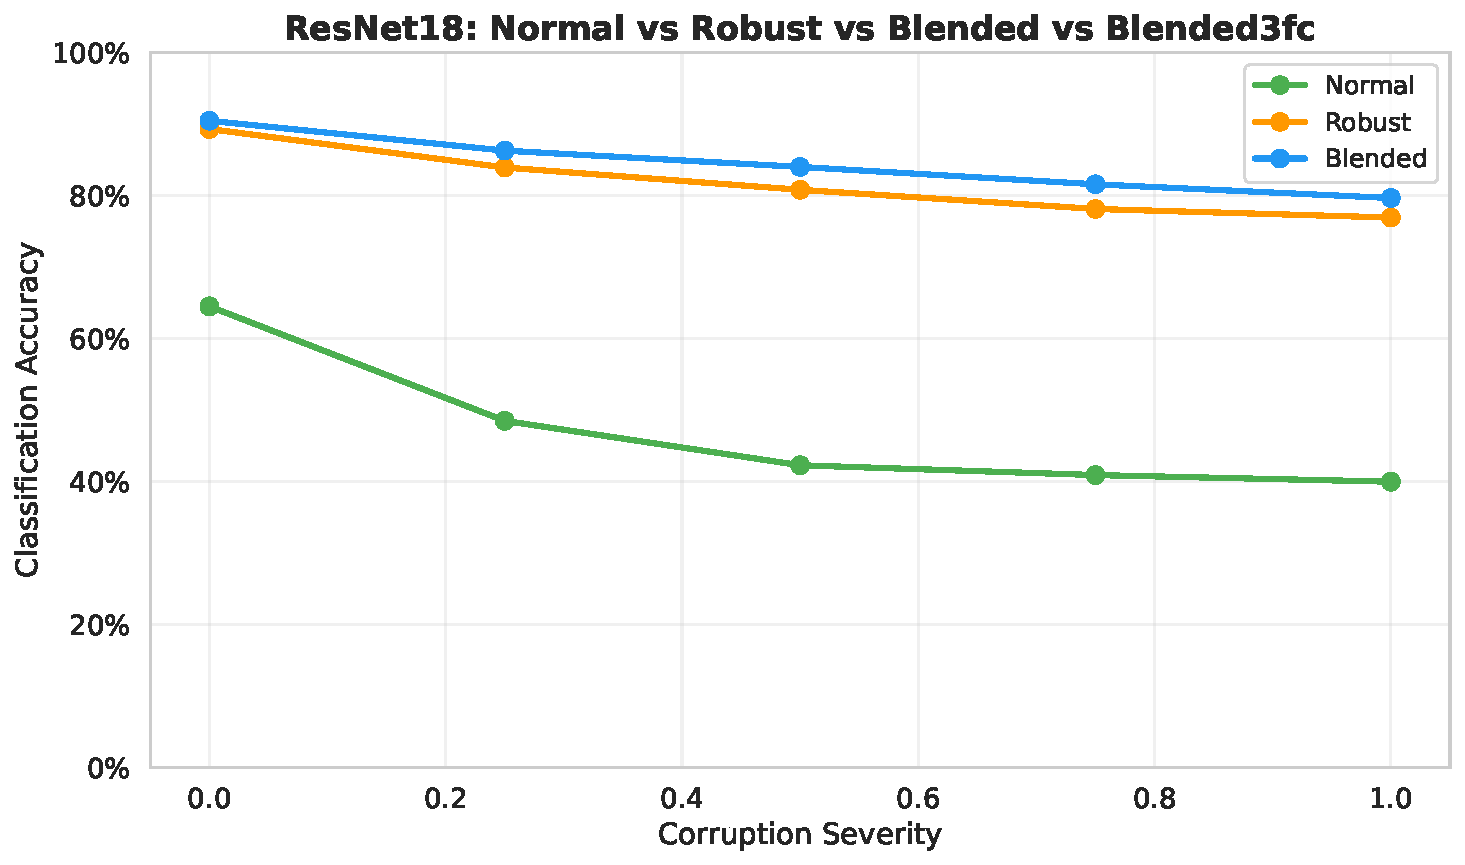
\includegraphics[width=\textwidth]{graphs/backbone_resnet18_comparison.pdf}
\caption{ResNet18}
\end{subfigure}
\hfill
\begin{subfigure}[b]{0.48\textwidth}
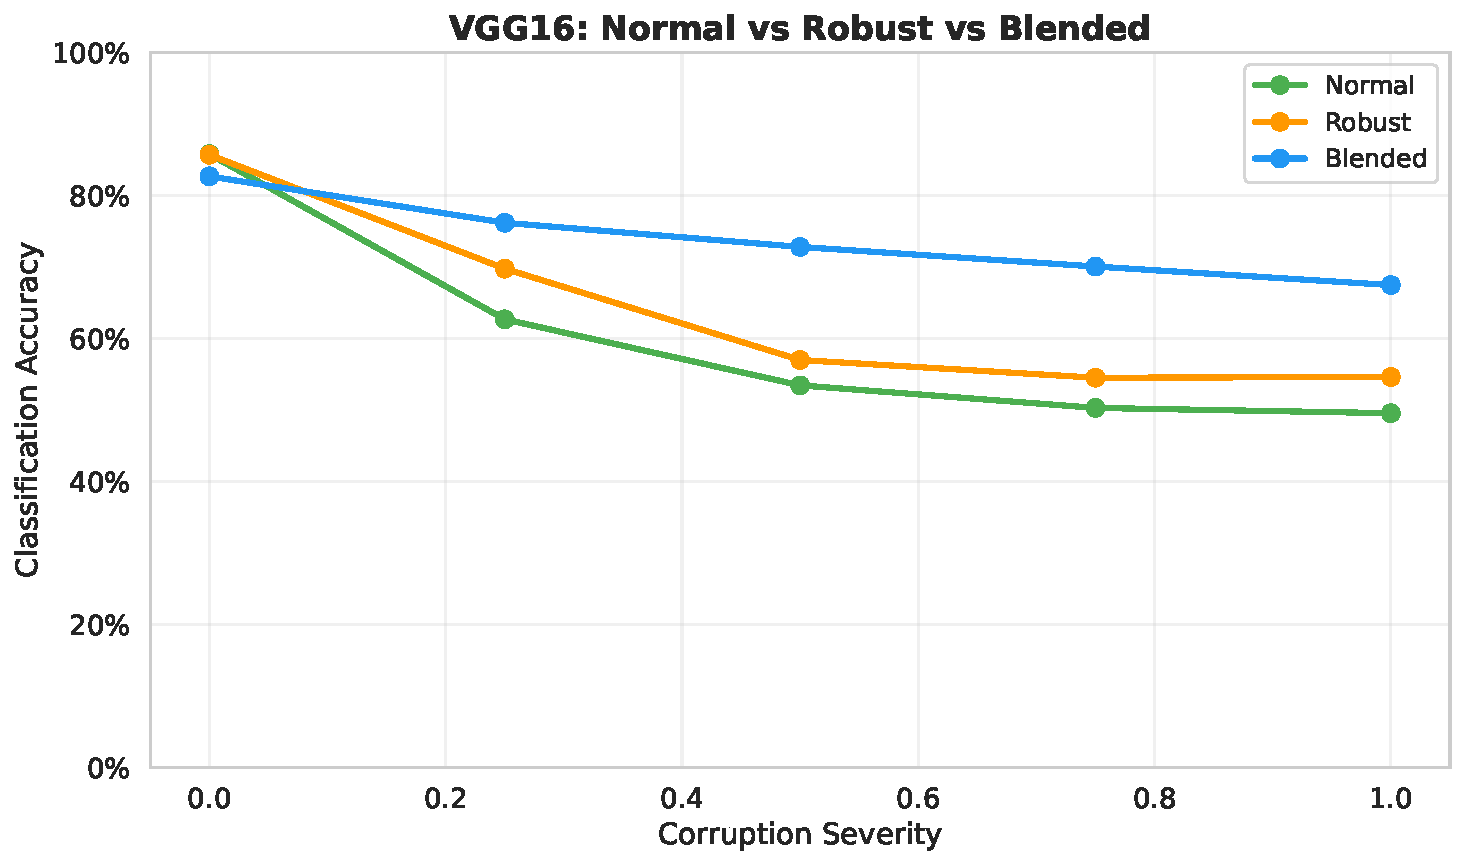
\includegraphics[width=\textwidth]{graphs/backbone_vgg16_comparison.pdf}
\caption{VGG16}
\end{subfigure}
\\[1em]
\begin{subfigure}[b]{0.48\textwidth}
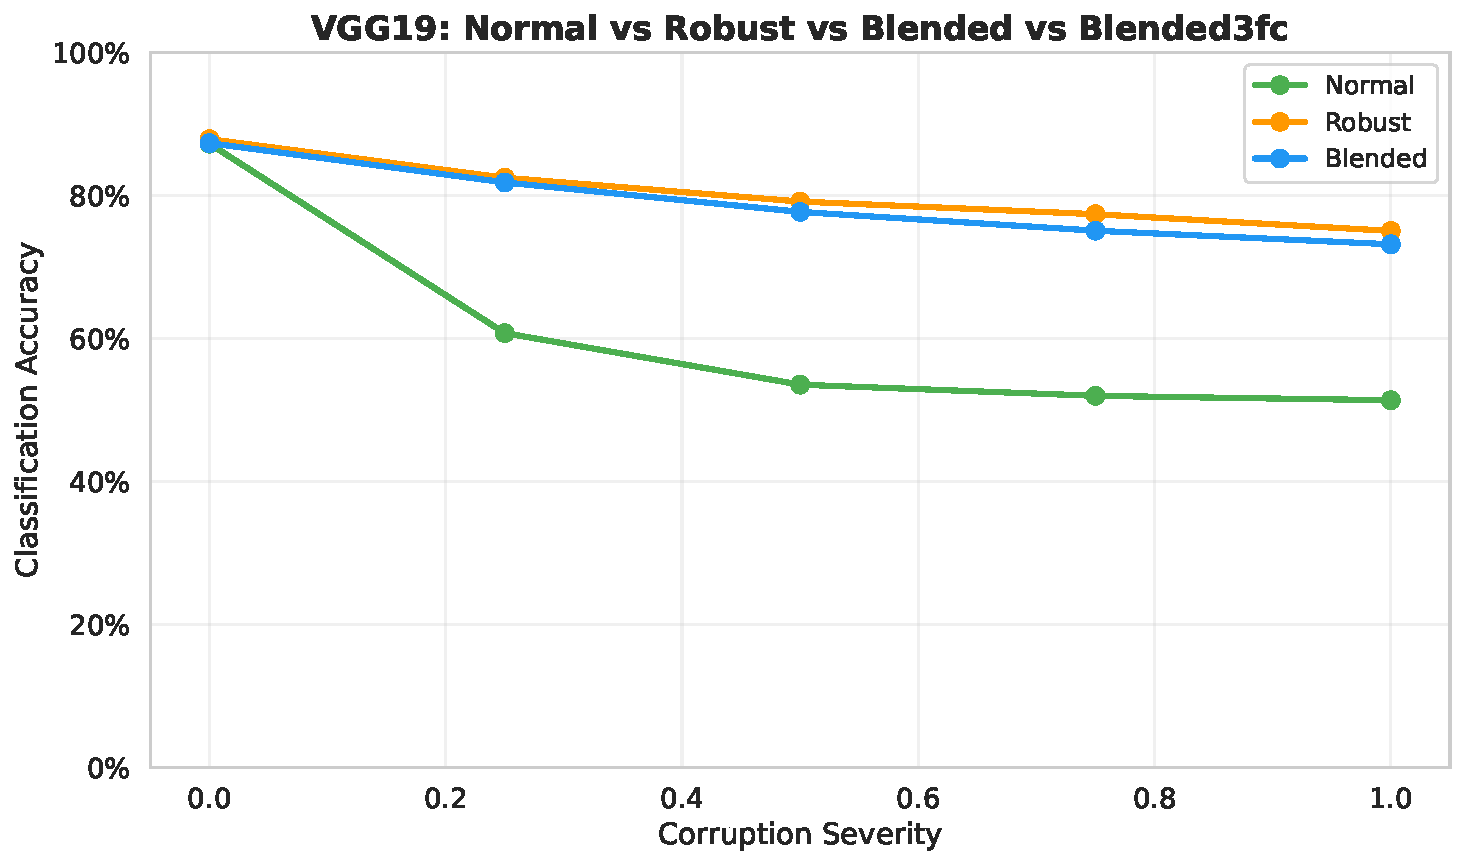
\includegraphics[width=\textwidth]{graphs/backbone_vgg19_comparison.pdf}
\caption{VGG19}
\end{subfigure}
\hfill
\begin{subfigure}[b]{0.48\textwidth}
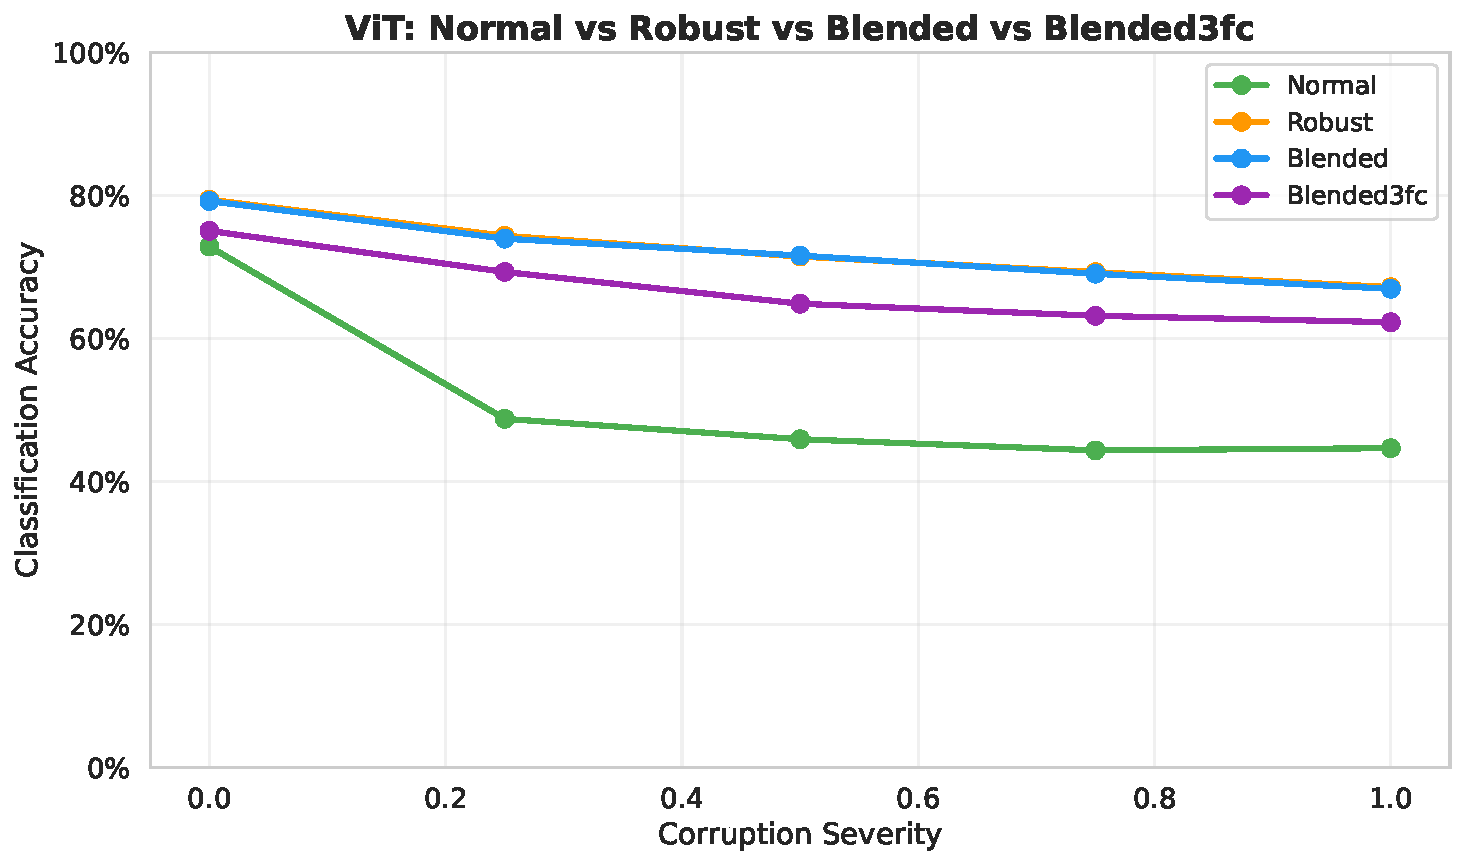
\includegraphics[width=\textwidth]{graphs/backbone_vit_comparison.pdf}
\caption{ViT}
\end{subfigure}
\\[1em]
\caption{Per-backbone comparison: Normal vs Robust vs Blended vs Blended3fc.}
\label{fig:per_backbone}
\end{figure}

\begin{figure}[H]
\centering
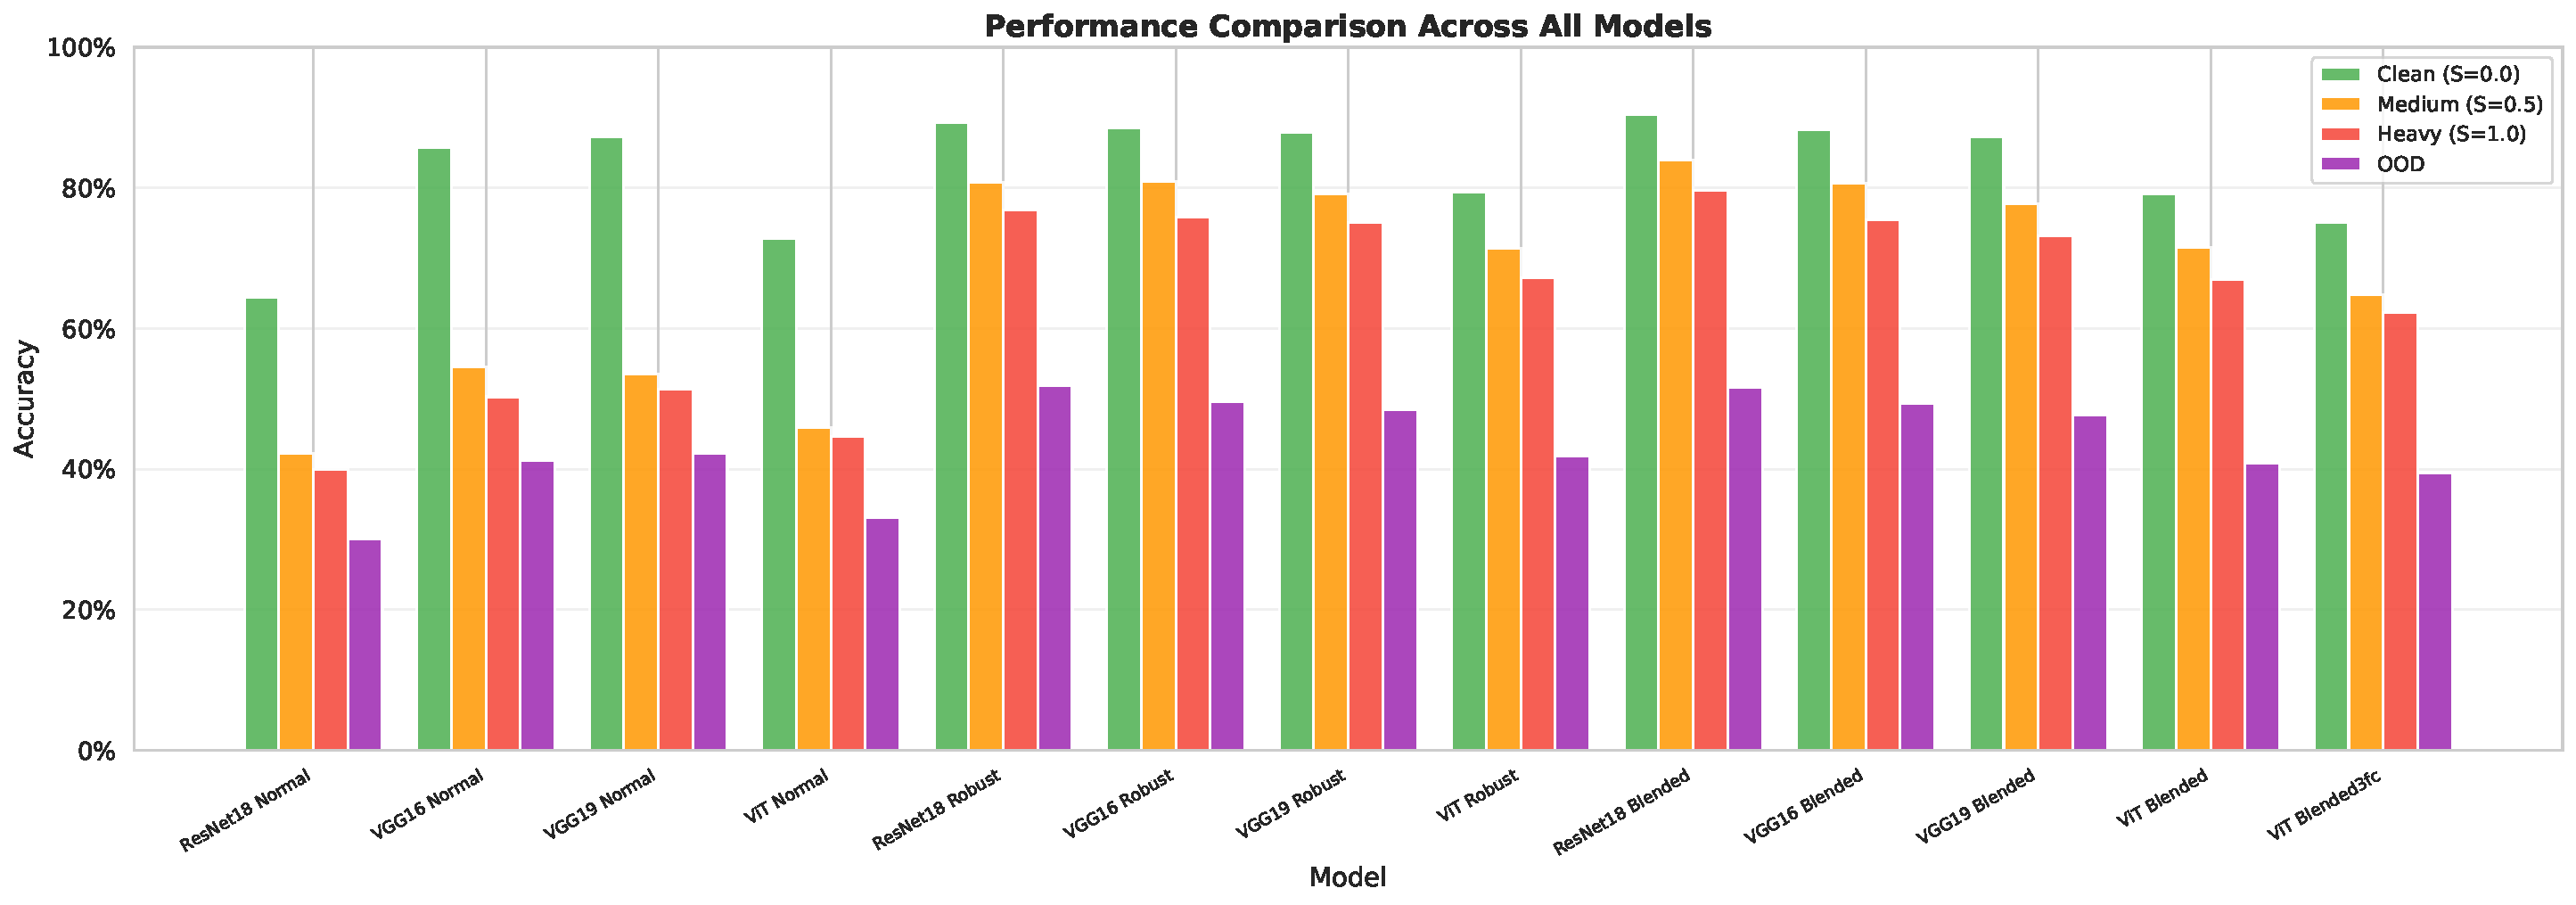
\includegraphics[width=0.95\textwidth]{graphs/overall_bar_comparison.pdf}
\caption{Performance comparison across all models and corruption levels.}
\label{fig:bar}
\end{figure}

\begin{figure}[H]
\centering
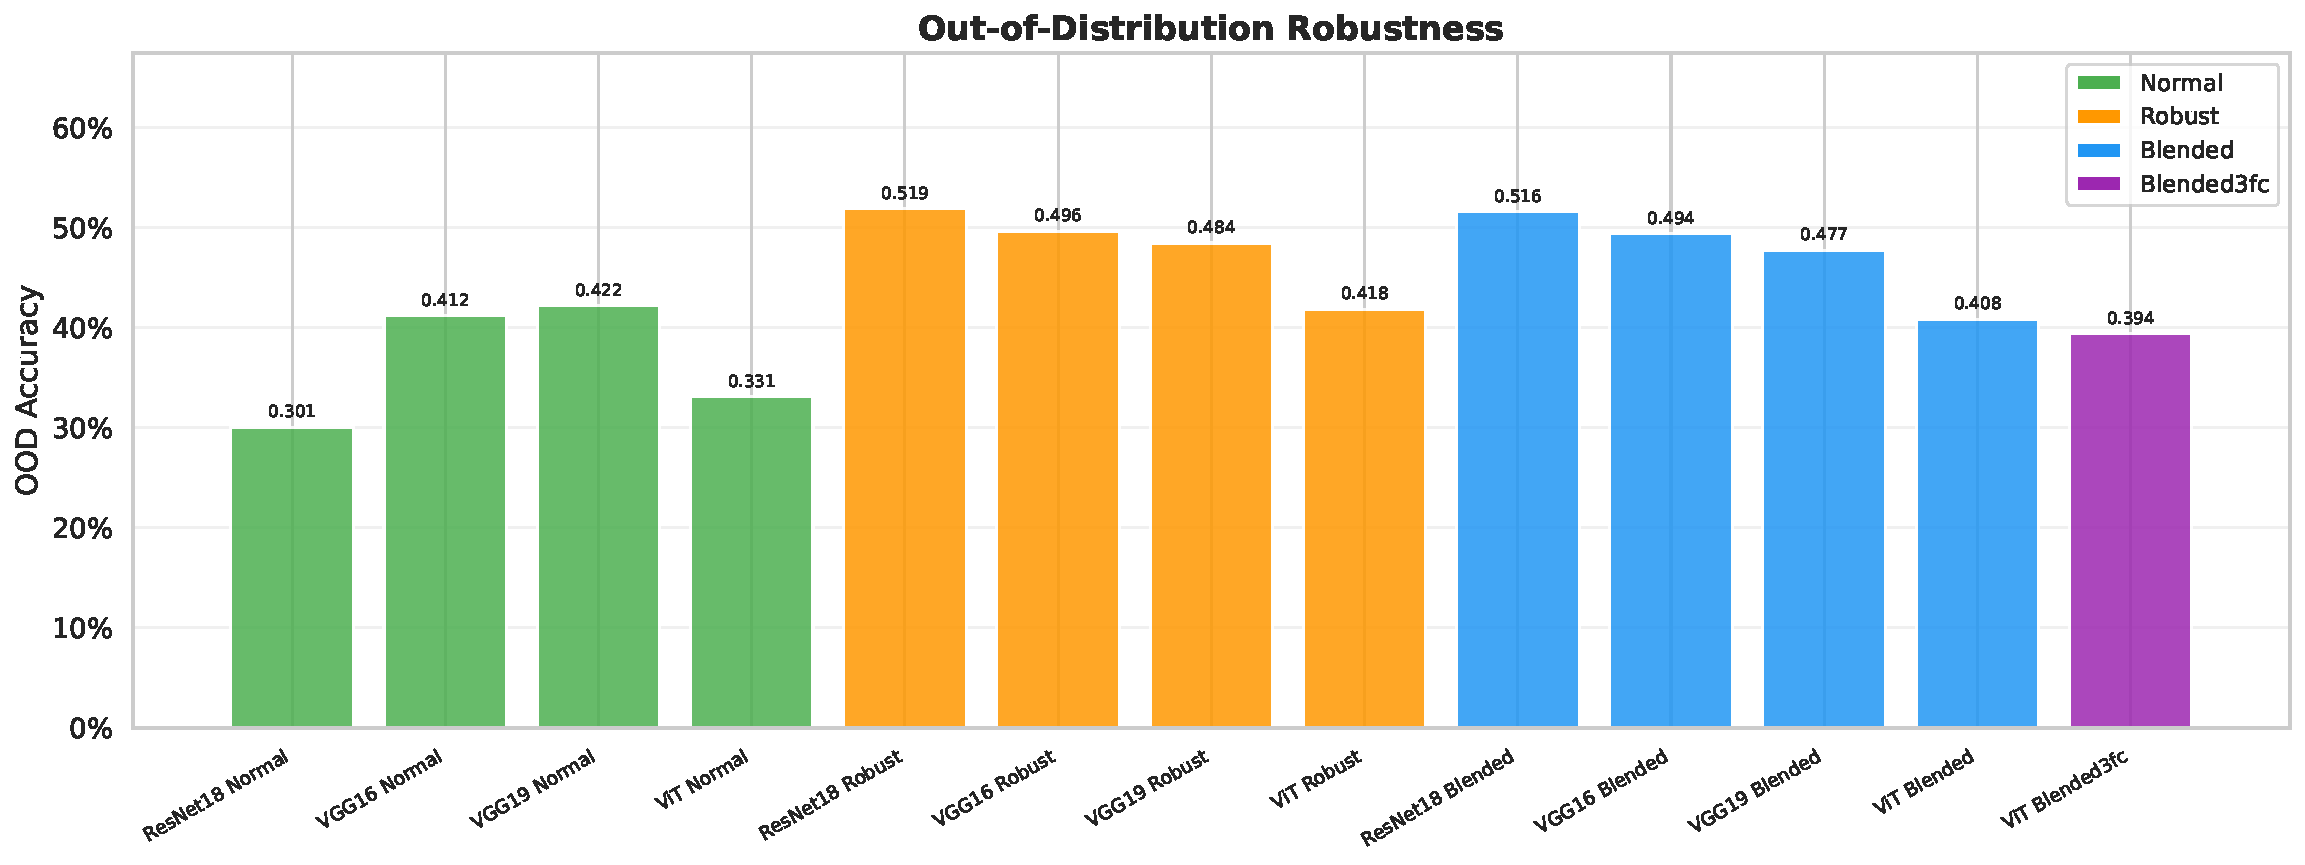
\includegraphics[width=0.85\textwidth]{graphs/overall_ood_comparison.pdf}
\caption{Out-of-distribution robustness comparison.}
\label{fig:ood}
\end{figure}

\begin{figure}[H]
\centering
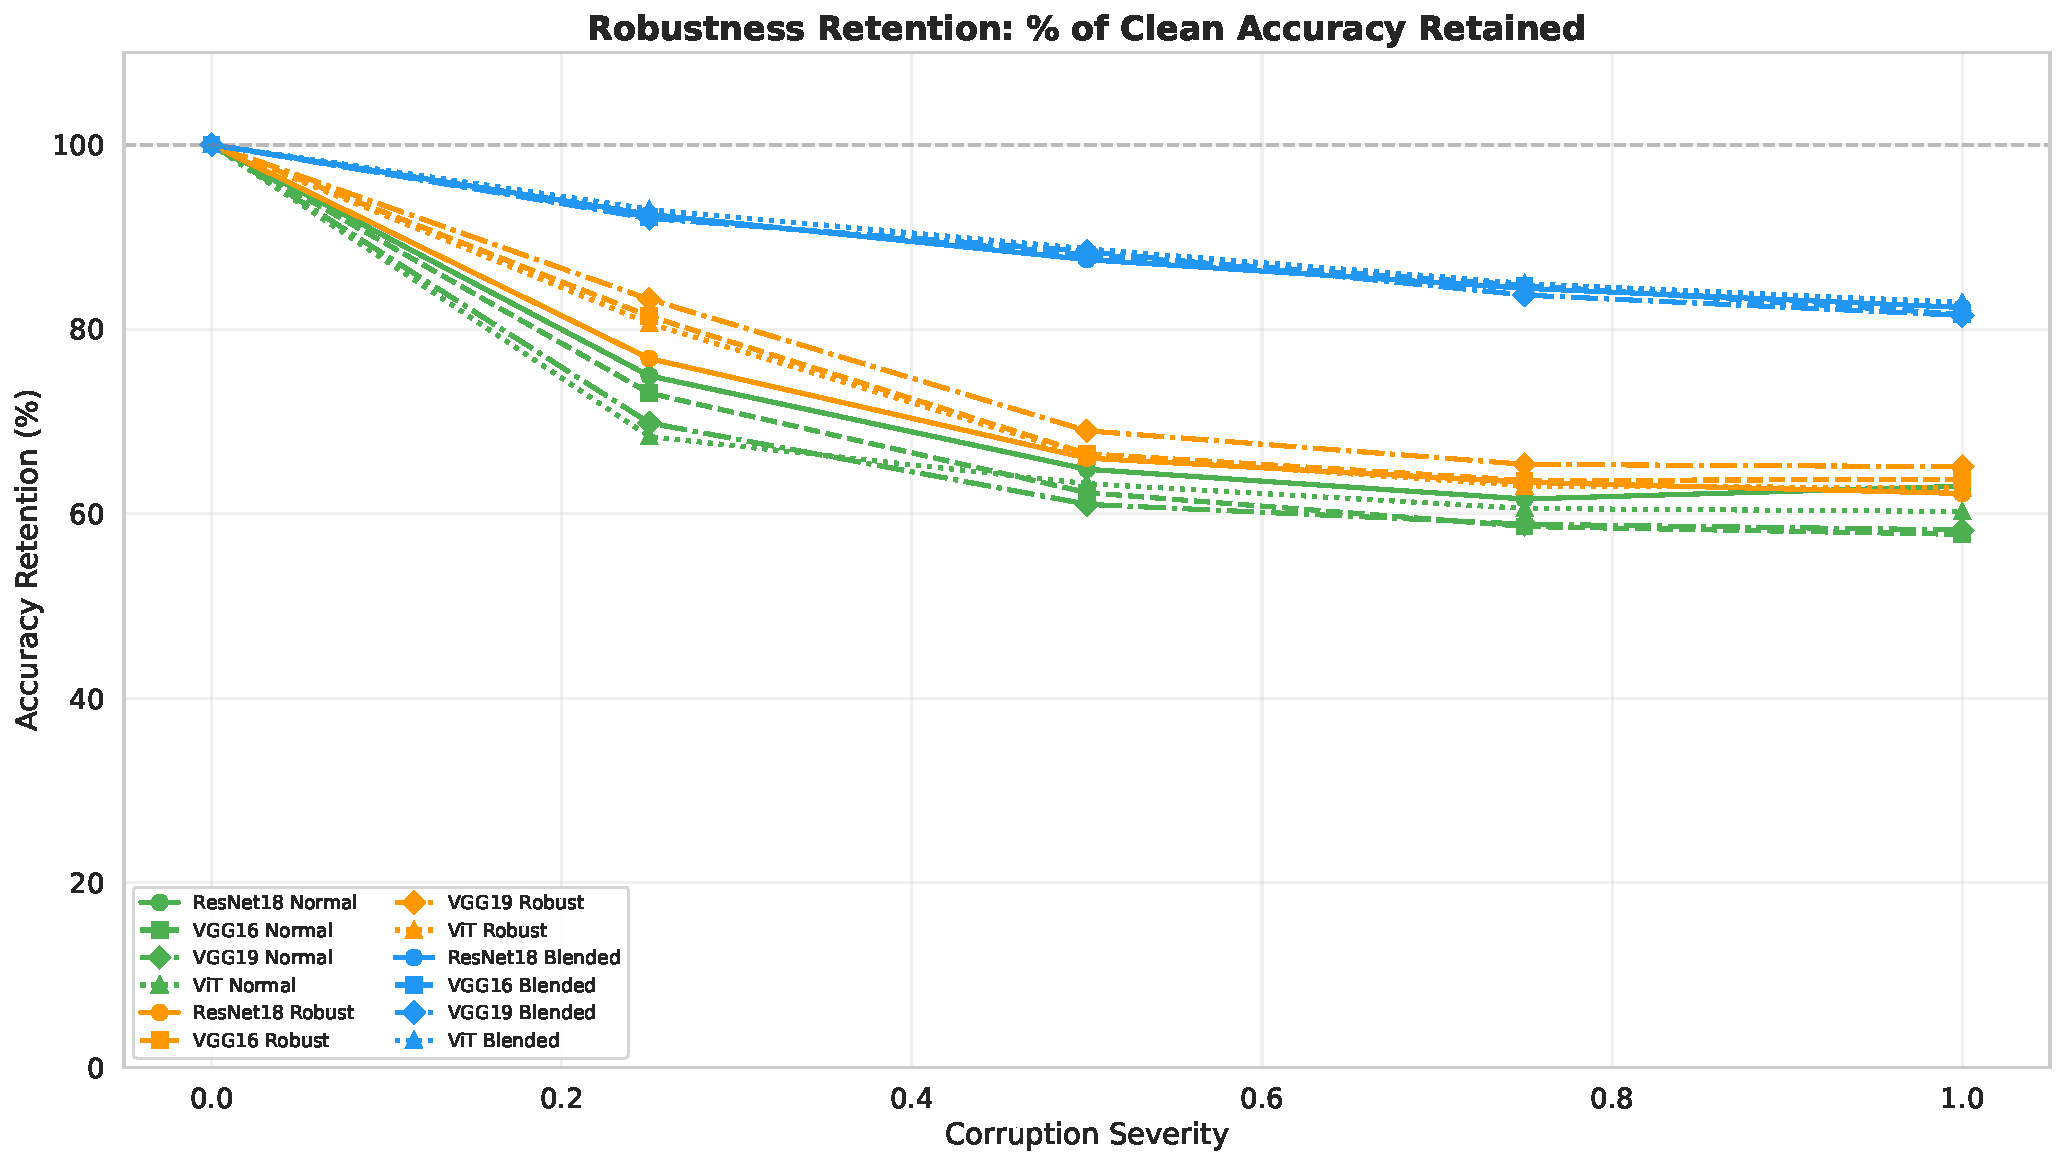
\includegraphics[width=0.85\textwidth]{graphs/robustness_retention.pdf}
\caption{Percentage of clean accuracy retained under corruption.}
\label{fig:retention}
\end{figure}

\section{Conclusion}
Our experiments demonstrate that predicting augmentation transforms with a minimal auxiliary loss consistently improves model robustness across all tested backbone architectures. The Blended models achieve lower accuracy degradation under corruptions and better out-of-distribution performance compared to both Normal (no augmentation) and Robust (augmented training) baselines.

\end{document}